\documentclass[letterpaper,10pt]{article}

\usepackage{enumitem}
\usepackage{titling}
\usepackage{listings,listings-rust}
\usepackage{url}
\usepackage{soul}
\usepackage{hyperref}
\usepackage{setspace}
\usepackage{subfig}
\usepackage{sectsty}
\usepackage{pdfpages}
\usepackage{colortbl}
\usepackage{multirow}
\usepackage{multicol}
\usepackage{relsize}
\usepackage{amsmath}
\usepackage{wasysym}
\usepackage{fancyvrb}
\usepackage[yyyymmdd]{datetime}
\usepackage{amsmath,amssymb,amsthm,graphicx,xspace}
\usepackage[titlenotnumbered,noend,noline]{algorithm2e}
\usepackage[compact]{titlesec}
\usepackage{XCharter}
\usepackage[T1]{fontenc}
\usepackage[scaled]{beramono}
\usepackage[normalem]{ulem}
\usepackage{booktabs}
\usepackage{tikz}
\usetikzlibrary{arrows.meta,automata,shapes,trees,matrix,chains,scopes,positioning,calc,decorations.pathreplacing}
\tikzstyle{block} = [rectangle, draw, fill=blue!20, 
    text width=2.5em, text centered, rounded corners, minimum height=2em]
\tikzstyle{bw} = [rectangle, draw, fill=blue!20, 
    text width=4em, text centered, rounded corners, minimum height=2em]

\definecolor{namerow}{cmyk}{.40,.40,.40,.40}
\definecolor{namecol}{cmyk}{.40,.40,.40,.40}
\renewcommand{\dateseparator}{-}

\let\LaTeXtitle\title
\renewcommand{\title}[1]{\LaTeXtitle{\textsf{#1}}}

\lstset{basicstyle=\footnotesize\ttfamily,breaklines=true}

\newcommand{\CPP}{C\nolinebreak\hspace{-.05em}\raisebox{.4ex}{\tiny\bf +}\nolinebreak\hspace{-.10em}\raisebox{.4ex}{\tiny\bf +}}
\def\CPP{{C\nolinebreak[4]\hspace{-.05em}\raisebox{.4ex}{\tiny\bf ++}}}

\newcommand{\handout}[5]{
  \noindent
  \begin{center}
  \framebox{
    \vbox{
      \hbox to 5.78in { {\bf ECE459: Programming for Performance } \hfill #2 }
      \vspace{4mm}
      \hbox to 5.78in { {\Large \hfill #4  \hfill} }
      \vspace{2mm}
      \hbox to 5.78in { {\em #3 \hfill \today} }
    }
  }
  \end{center}
  \vspace*{4mm}
}

\newcommand{\lecture}[3]{\handout{#1}{#2}{#3}{Lecture#1}}
\newcommand{\tuple}[1]{\ensuremath{\left\langle #1 \right\rangle}\xspace}

\addtolength{\oddsidemargin}{-1.000in}
\addtolength{\evensidemargin}{-0.500in}
\addtolength{\textwidth}{2.0in}
\addtolength{\topmargin}{-1.000in}
\addtolength{\textheight}{1.75in}
\addtolength{\parskip}{\baselineskip}
\setlength{\parindent}{0in}
\renewcommand{\baselinestretch}{1.5}
\newcommand{\term}{Winter 2020}

\singlespace


\begin{document}

\lecture{14 --- Early Termination, Reduced-Resource Computation}{\term}{Jeff Zarnett \& Patrick Lam}

\section*{Trading Accuracy for Time}

Knowing when to quit is wise. In some cases, we can speed up our program by not waiting for the slowest steps to be done. This is somewhat related to speculation, but the big distinction is that in speculation we do extra work ``just in case'' and with early phase termination, we skip doing some work even though we're supposed to do on the basis of ``close enough is good enough''.  There are two basic ideas: the first way is to skip some parts of work and the second is to intentionally reduce accuracy to speed things up. 

You may implement these strategies when you're writing an exam: time is limited and you might choose not to do a certain question because the benefit is small and you can use your time better doing a different question. In which case you might leave question 3.2 blank in favour of working on question 4.1. That's where you skip some work. Alternatively, you could choose to skip error handling in question 4.1, knowing that you will lose some marks in that question but freeing up some more time to do question 3.2. Exams are nice (or nasty) in that we can do both things, but your program might support only one.

\subsection*{Early Phase Termination}

The formal name for the first idea, quitting early, is is early phase
termination~\cite{Rinard:2007:EarlyPhaseTermination}. So, to apply it to a concrete idea: we've talked about barriers quite a bit. Recall that the idea is that
no thread may proceed past a barrier until all of the threads
reach the barrier. Waiting for other threads causes delays. 
Killing slow threads obviously speeds up the program. Well, that's easy.

\begin{center}
``Oh no, that's going to change the meaning of the program!''
\end{center}

Let's consider some arguments about when it may be acceptable to just
kill (discard) tasks. Since we're not completely crazy, we can develop
a statistical model of the program behaviour, and make sure that the
tasks we kill don't introduce unacceptable distortions. Then when we
run the program, we get an output and a confidence interval.

If you wanted a game-relevant example, pretend you're really bad at Mario Kart. If you're in last place when the second-last player (or AI) drives across the finish line, the race is over at that point because we already know you finished last (``Oh nooo!''). There's no benefit to waiting while you have to drive the rest of the lap to the finish. In that case, ending the race while one driver has not yet finished is perfectly safe because the outcome is already known: I'm really bad at Mario Kart.

\paragraph{Should Have Made A Left Turn At Albuquerque.} 
Many problems are mathematically hard in nature: to find the optimal solution you have to consider every possibility. Well, what this strategy presupposes is: don't. Imagine the travelling salesperson problem, just for the sake of an example. There are $n$ points to visit and you want to minimize the amount of travel time. The only way to know if a solution is best is to consider every possible route.

One way we can know if we're wasting time is to remember previous outcomes. The solution we're evaluating will have some travel cost in units (maybe kms). If the currently-accumulated cost in kms is larger than the total of the thus-far best solution, give up. To be specific, if we have a route that has 400 km of driving and we are partway through building a solution and we have already got 412 km of driving, we can give up on this option (and not evaluate the rest of it) because we already know it won't be the best.

Another approach is to stop as soon as you have a solution that's reasonable. If our target is to get total travel under 500 km then we can stop searching as soon as we find one that satisfies this constraint. Yes, we might stop at 499 km and the optimal solution might be 400 (25\% more driving for the poor peon) -- but it does not have to be perfect; it just has to be acceptable. And if traffic in the hypothetical region is anything like that of the GTA, the route that is shortest in kilometres may not be the shortest in terms of time anyway.

You can also choose to reduce the amount of effort by trying, say, five or ten different possibilities and seeing which of those is the best. There's no guarantee you'll get an optimal solution: you might have randomly chosen the ten worst options you could choose. 

Interesting to think about: what does Google Maps do? For some problems there are relatively few solutions; if you plan to drive in the Yukon territory there are a finite set of roads to travel. But suppose you're driving around Toronto; the grid system means there are lots and lots of options, right? Maybe some heuristic is used to generate some possibilities and the best ones of those are chosen.


\paragraph{This Point is Too Hard.} Monte Carlo simulations
are a good candidate; you're already picking points randomly.
Raytracers can work as well. Both of these examples could spawn a lot
of threads and wait for all threads to complete. For mathematical functions that are ``not nice'', different points might take longer to evaluate than others. 
In either case, you
can compensate for missing data points, assuming that they look similar to
the ones that you did compute. If you have a function where some graph is being
computed, you can probably guess that a missing point is somewhere in between the two (or $n$) nearest points. So just average them.

The same is true for graphics, of course: if rendering a particular pixel did
not go well for some reason, you can just average the adjacent ones and probably
people would not notice the difference. Not bad!

In other cases, some threads simply take too long, but we don't need all of them to produce a result. If we are evaluating some protocol where the majority wins, we can stop as soon as sufficient results have been returned; either an outright majority for an option or that the remaining votes couldn't change the outcome. This happens to some extent with election projections: even if not all polling stations are reporting a result, news channels will declare a winner if the remaining votes would not be enough to change the outcome. Actually, news channels probably take it a bit too far in that they will declare a winner even if the outstanding votes exceed the margin, on a theory that it probably won't be the case that they are 100\% for the candidate who is in second place. But they can be wrong.

\paragraph{Slow Road...}
For some categories of problem, we know not only that a solution will exist, but also how many steps it takes to solve (optimally). Consider the Rubik's Cube -- it's much easier to explain if you have seen one. It'll appear in the slides, but if you're just reading the note(book/s) then I suggest you google it\footnote{If you've waited for the exam to read this and you can't google... whoops!}.

This is a problem with a huge number of possible permutations and brute force isn't going to work. However, research has proven that no matter what the state of the cube is, it can be transitioned to a solved state in 20 moves or fewer. This number is called God's Number, presumably because it is the maximum number of moves it would take an all-knowing deity to solve the puzzle. So if you have a solver for a Rubik's cube, and if you don't find a solution in (fewer than) 20 moves, you should cancel this solution attempt and try another one.

Okay, that's fun to talk about, but it's always better if we see it in action? Let's play around with \url{https://rubiks-cube-solver.com/}, which implements this very behaviour. It says in their description of how it works that it runs an open source algorithm; it looks for a solution in 20 steps or fewer. This implementation does both kinds of tradeoff: if the solution being evaluated takes too long it's killed. And if no under-20-move solution has been found within a certain time limit, it will return a solution that takes 24 steps and give you a less optimal solution. That's actually an example of reducing accuracy (quality of solution) for speed, which leads us into our next approach.

\subsection*{Reduced-Resource Computation}

The formal name for the second idea is ``reduced resource computation'' -- that is to say, we do more with less! Austerity programs for our computer programs. Well, you can use \texttt{float} instead of \texttt{double}. But you can also work with integers to represent floating point numbers (e.g., representing money in an integer number of cents). But let's really  think about when this is appropriate.

\paragraph{Circuit... Analysis!} Recall that, in scientific computations, you're entering points that were measured (with some error) and that you're computing using machine numbers (also with some error). Computers are only providing simulations, not the ground truth; the question is whether the simulation is good enough.

Imagine that the simulation is deciding on what resistors are going to be put in your circuit board: is there any point in calculating it down to five decimal places when the resistors you buy have a tolerance of $\pm$5\%? No, and if you took a circuits course with Prof. Barby he would be very disappointed if you said yes.


\paragraph{iddqd.} Perhaps my favourite example of trading accuracy for time is a function in Quake III, contributed by John Carmack known as ``fast inverse square root''. For graphics processing, sometimes you want to calculate $1/\sqrt{x}$. This is important because you use it in calculating lighting and reflections (because you normalize vectors). Normalizing is mostly a straightforward exercise: square some numbers, add them up, and then... oh no, you have to use square root... That one isn't so simple.

Square root (or similar) is usually calculated by some interpolation or root-finding method (if you took a numerical methods course, you know several techniques for calculating this). But instead there's this~\cite{fisqrt}. 

\begin{lstlisting}[language=C]
float FastInvSqrt(float x) {
  float xhalf = 0.5f * x;
  int i = *(int*)&x;         // evil floating point bit level hacking
  i = 0x5f3759df - (i >> 1);  // what the fuck?
  x = *(float*)&i;
  x = x*(1.5f-(xhalf*x*x));
  return x;
}
\end{lstlisting}

The first line of the function is straightforward - take half the value of \texttt{x}. The second one says to interpret the value of \texttt{x} as an \texttt{int}. Now this probably seems like dark magic, and it is. Pretend this floating point number is an integer. I mean, you can, but why does this make sense? 

There's a lot of explanation and a lot of math in the source material but it comes down to how the float is stored. The float starts with a sign bit, then the exponent, and then the mantissa (math reminder: in $1.95 \times 10^{3}$, the exponent is 3 and the mantissa is 1.95).

The clever hack is somewhat obsoleted now by the fact that CPU instructions now exist to give you fast inverse square root. This was obviously not something you could rely on in 1999, but we're going to revisit the idea of using clever CPU instructions to speed things along in the next lecture. So if we say pretend this float is an integer we end up with this~\cite{fisqrt2}:

\begin{center}
	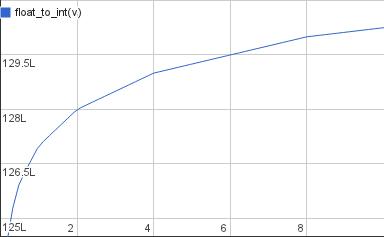
\includegraphics[width=0.4\textwidth]{images/float-to-int.png}
\end{center}

If it's not obvious, this plot rather resembles the plot of $-1/\sqrt{x}$. So we are pretty close to getting where we need to go. All we need is to invert it and then do a little bit of an offset. The seemingly magic number of \texttt{0x5f3759df} is not a bit pattern, but just a calculated offset to make the approximation a little bit better. Then we turn it back into a float.

The last step is then to do one quick iteration of Newton's method to refine the calculation a little bit and we have a great solution: it is a fast, constant-time calculation for something that normally would be difficult, and it's very accurate, something like 0.175\% error at the most. And in a 3D game a tiny inaccuracy is not a big deal! Especially in one from 1999. It wasn't exactly photorealistic to begin with, now was it...?

This is the best case scenario: the accuracy that we trade for speed is both very small and its application is one in which a small difference is not noticeable. This is beyond ``close enough is good enough'', this is hardly any tradeoff at all.


\paragraph{N-Body Problem}
A common physics problem that programmers are asked to simulate is the N-Body problem: you have some number of bodies (N!) and they interact via gravitational forces. The program needs to compute the movements of the bodies over time. This is a typical example of a program that is well suited to parallelization: you can compute the forces on each body $n$ from all other bodies in parallel. This was even at one time an OpenCL assignment in this course, although now there are too many good solutions on the internet so it was replaced. Bummer.

What can you do here if you want to speed it up even more? You could look for optimizations that trade off accuracy for performance. As you might imagine, using \texttt{float} instead of \texttt{double} can save half the space which should make things quite a bit faster. But you want more...

Then we need some domain knowledge. That is, we need to think about what we know about the problem and we can make a decision about what is important and what is not. If we thought about what's important for determining the forces, what would we consider to be the most important? 

Hint: consider the formula: $F = \dfrac{Gm_{1}m_{2}}{r^{2}}$. 

Force is a function of how close the objects are. Thus, points that are far away contribute only small forces. So you can estimate them (crudely). A first approximation might say that forces that are far enough away are zero. In principle, Jupiter has a gravitational influence on the rate of descent if I drop a whiteboard marker (whether positive, negative, or zero depends on its relative position at the time of my clumsiness), but the effect is so incredibly small as to be worth ignoring. But what about objects that are not exactly close by, but also not so far away as to be irrelevant?

The idea is to divide the points into a number of ``bins'' which are cubes representing a locale of some sort. Then, compute the centre of mass for each bin. When calculating the forces on a given point, add the force exerted by the centre of mass for faraway bins to the force exerted by individual particles for nearby particles.

A more concrete explanation with an example: suppose the space  is divided into $[0, 1000]^3$, so we can take bins which are cubes of length 100. This gives 1000 bins. If you want to increase the accuracy, increase the number of bins. If you want to increase the speed, decrease the number of bins: either make bins larger, or change your definition of what is too far away to care about.

The program should have a 3-dimensional array {\tt cm} of a point structure to store centres-of-mass. The {\tt x}, {\tt y} and {\tt z}
components contain the average position of the centres of mass of a
bin, while the {\tt w} component stores the total mass. Compute all of
the masses in parallel: create one thread per bin, and add a point's
position if it belongs to the bin, e.g.

\begin{lstlisting}
    int xbin, ybin, zbin; // initialize with bin coordinates
    int b;
    for (i = 0; i < POINTS; i++) {
        if (pts[i] in bin coordinates) {
            cm[b].x += pts[i].x; // y, z too
            cm[b].w += 1.0f;
        }
    }
    cm[b].x /= cm[b].w; // etc
\end{lstlisting}

 \noindent
Note that this parallelizes with the number of bins.

For the next step, the program needs to keep track of the points in
each bin. Fortunately, you've collected the number of points in each
bin, so you can allocate the appropriate amount of memory to store the
points in a two-dimensional array {\tt binPts}. In a second phase,
iterate over all bins again, this time putting coordinates into the
proper element of {\tt binPts}.


The payoff from all these calculations is to save time while
calculating forces. In this example, we'll compute exact
forces for the points in the same bin and the directly-adjacent bins
in each direction (think of a Rubik's Cube; that makes 27 bins in all,
with 6 bins sharing a square, 12 bins sharing an edge, and 8 bins
sharing a point with the centre bin). If there is no adjacent bin 
(i.e., this is an edge), just act as if there are no points 
in the place where the nonexistent bin would be. 

This does mean there is overhead for each step, meaning the total amount of overhead goes up. Is it worth it? Let's see the data from a reference solution [PL] for the previous assignment, implemented in OpenCL (i.e., run on the GPU):

\paragraph{With 500*64 points.}
\begin{itemize}
\item    OpenCL, no approximations (1 kernel): 0.182s
\item    OpenCL, with approximations (3 kernels): 0.168s
\end{itemize}
 \paragraph{With 5000*64 points.}
\begin{itemize}
\item    OpenCL, no approximations (1 kernel): 6.131s
\item    OpenCL, with approximations (3 kernels): 3.506s
\end{itemize}


\subsection*{Loop perforation} 
You can also apply the same idea to sequential programs. Instead
of discarding tasks, the idea here is to discard loop iterations~\cite{hoffmann09:_using_code_perfor_improv_perfor}.
Here's a simple example: instead of the loop,
\begin{center}
\verb|for (i = 0; i < n; i++) sum += numbers[i];|
\end{center} \vspace*{-1em}
simply write,
\vspace*{-1em}\begin{center}
\verb|for (i = 0; i < n; i += 2) sum += numbers[i];|
\end{center}
and multiply the end result by a factor of 2. This only works 
if the inputs are appropriately distributed, but it does give a
factor 2 speedup.

\paragraph{Example domains.} In~\cite{Rinard:2010:PSA:1932682.1869525},
we can read that loop perforation works for evaluating forces on water
molecules (in particular, summing numbers); Monte-Carlo simulation for
swaption pricing; and video encoding. In that example, changing loop
increments from 4 to 8 gives a speedup of 1.67, a signal to noise ratio
decrease of $0.87\%$, and a bitrate increase of $18.47\%$, producing
visually indistinguishable results. The computation looks like this:

{\small
\begin{verbatim}
min = DBL_MAX;
index = 0;
for (i = 0; i < m; i++) {
  sum = 0;
  for (j = 0; j < n; j++) sum += numbers[i][j];
  if (min < sum) {
    min = sum;
    index = i;
  }
}
\end{verbatim}
}
The optimization changes the loop increments and then compensates. 


\bibliographystyle{alphaurl}
\bibliography{459}


\end{document}
